\pagebreak

\section{Time Series Results}

Figures \ref{fig:averageKF0} - \ref{fig:averageCombn0} were generated by feeding the time series data into our Kalman Filter (KF) and Weighted Least Squares (WLS) methods with varying $Q$ and $\lambda$ parameters respectively. In these graphs, both methods predicted final percent-fill by averaging the predictions from all 15 KF and WLS respectively.

\begin{figure}[h]
\centering
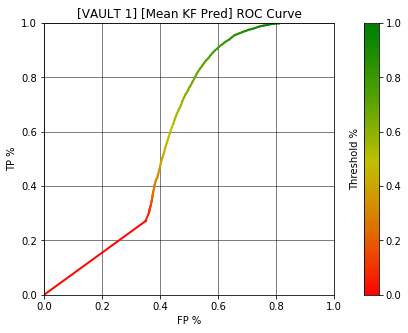
\includegraphics[width=8cm]{body/results/Graphs/JustSeries/1.PerformaceofMean/1.KF/Raw/v1.png}
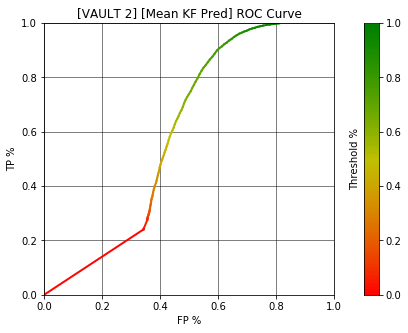
\includegraphics[width=8cm]{body/results/Graphs/JustSeries/1.PerformaceofMean/1.KF/Raw/v2.png}
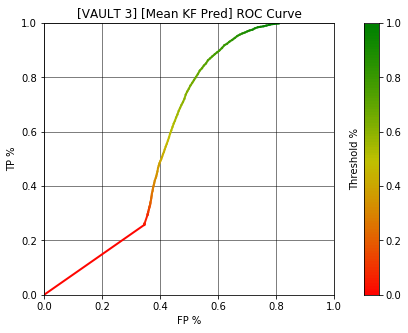
\includegraphics[width=8cm]{body/results/Graphs/JustSeries/1.PerformaceofMean/1.KF/Raw/v3.png}
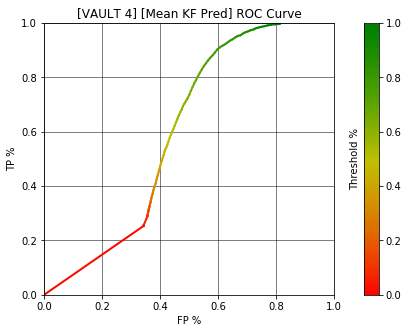
\includegraphics[width=8cm]{body/results/Graphs/JustSeries/1.PerformaceofMean/1.KF/Raw/v4.png}
\caption{ROCs generated based on the average percent-fill prediction of all 15 of our KF's on the entirety of each validation set. Top Left: Validation set 1. Top Right: Validation set 2. Bottom Left: Validation set 3. Bottom Right: Validation set 4.}
\label{fig:averageKF0}
\end{figure}

\pagebreak

\begin{figure}[h]
\centering
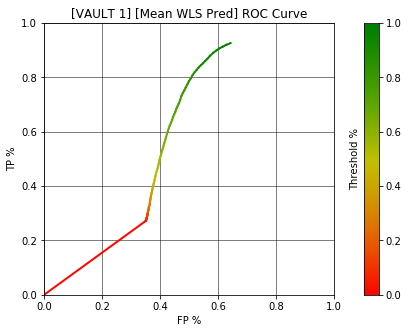
\includegraphics[width=8cm]{body/results/Graphs/JustSeries/1.PerformaceofMean/2.WLS/Raw/v1.png}
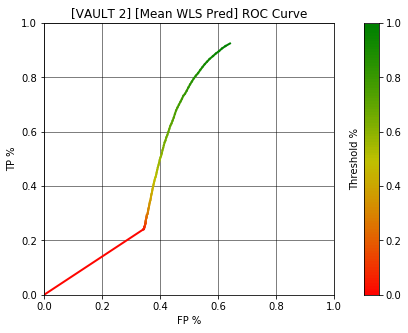
\includegraphics[width=8cm]{body/results/Graphs/JustSeries/1.PerformaceofMean/2.WLS/Raw/v2.png}
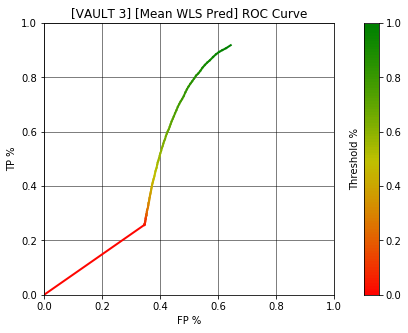
\includegraphics[width=8cm]{body/results/Graphs/JustSeries/1.PerformaceofMean/2.WLS/Raw/v3.png}
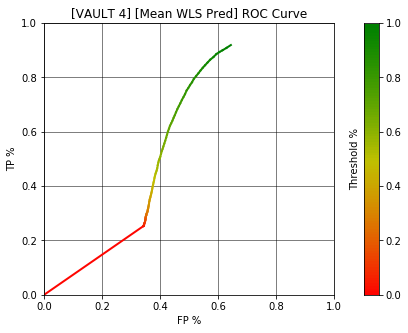
\includegraphics[width=8cm]{body/results/Graphs/JustSeries/1.PerformaceofMean/2.WLS/Raw/v4.png}
\caption{ROCs generated based on the average percent-fill prediction of all 15 of our KF's on the entirety of each validation set. Top Left: Validation set 1. Top Right: Validation set 2. Bottom Left: Validation set 3. Bottom Right: Validation set 4.}
\label{fig:averageWLS0}
\end{figure}

Figure \ref{fig:averageKF0} shows the result of using the averaged percent-fill predictions of all 15 KF's on all 4 validation sets. Similarly, Figure \ref{fig:averageWLS0} shows the result of using the averaged percent-fill predictions of all 15 WLS's on all 4 validation sets. Immediately, we can see the averaged prediction of our 15 KF and WLS independently perform worse than even the baseline from Figure \ref{fig:baseline}. A direct comparison of all three can be found in Figure \ref{fig:averageComp0}. It should be noted that KF and WLS produce nearly identical curves, with KF tending to perform very slightly better in the False Positive range of around 0.4 - 0.5. This may imply both methods are equal or very nearly equal in terms of predictive performance. This would be expected as both perform an exponential fit on the data, just in different ways.

\pagebreak

\begin{figure}[h]
\centering
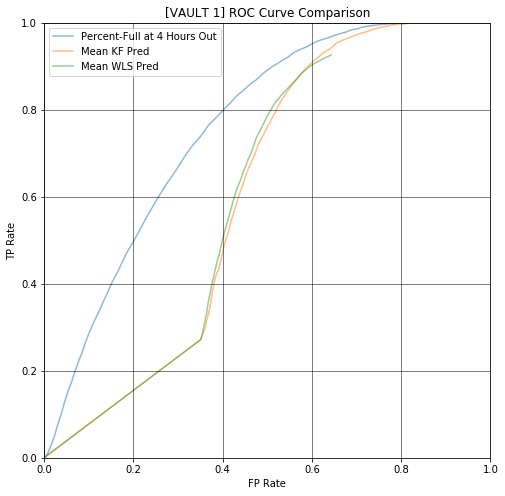
\includegraphics[width=7cm]{body/results/Graphs/JustSeries/1.PerformaceofMean/3.Compare/Raw/v1.png}
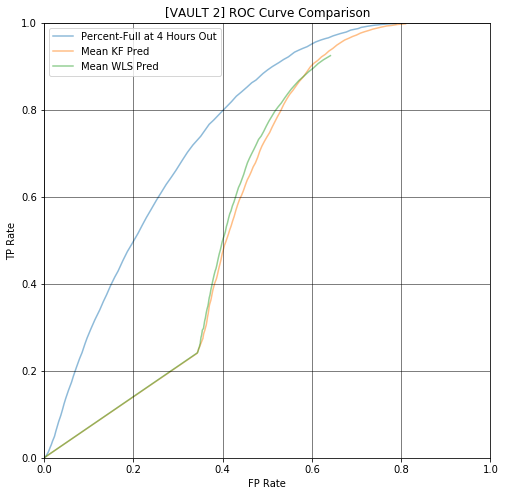
\includegraphics[width=7cm]{body/results/Graphs/JustSeries/1.PerformaceofMean/3.Compare/Raw/v2.png}
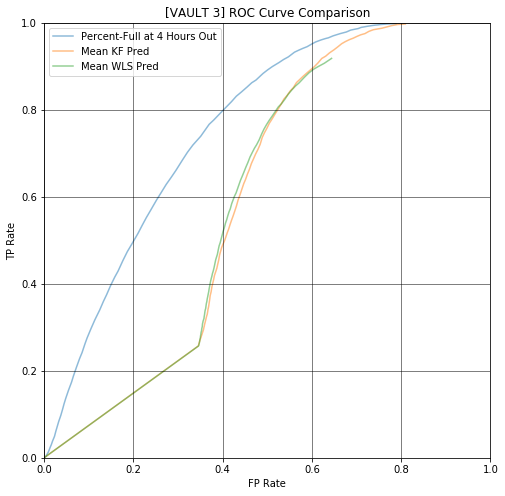
\includegraphics[width=7cm]{body/results/Graphs/JustSeries/1.PerformaceofMean/3.Compare/Raw/v3.png}
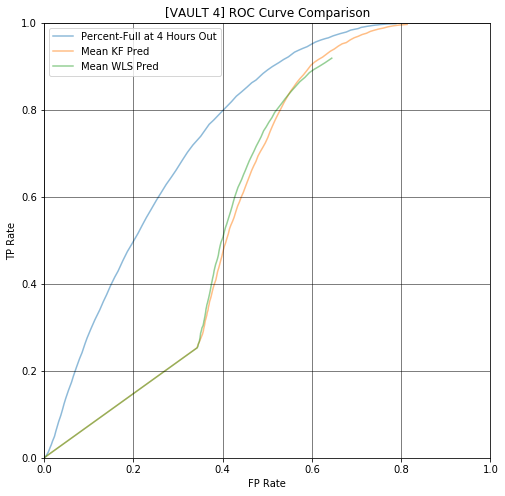
\includegraphics[width=7cm]{body/results/Graphs/JustSeries/1.PerformaceofMean/3.Compare/Raw/v4.png}
\caption{ROCs generated based on the average percent-fill prediction of all 15 of our KF's on the entirety of each validation set. Top Left: Validation set 1. Top Right: Validation set 2. Bottom Left: Validation set 3. Bottom Right: Validation set 4.}
\label{fig:averageComp0}
\end{figure}

One thing all these graphics share is a long, straight initial section in the curves. We believed this piece appeared because there were a large portion of contests which had no time series data available before the ``4 Hour Out'' point. This meant the KF and WLS could not make any predictions as they had no starting data. In order to get a better sense for how well averaging the KF and WLS predictions performs, we recreated Figures \ref{fig:averageKF0} - \ref{fig:averageComb0} considering only contests which had data before the ``4 Hour Out'' point. The results of limiting to only ``non-zero'' data as we call it, (contests with data before ``4 Hours Out'') can be found in Figures \ref{fig:averageKFn0} - \ref{fig:averageCombn0}.

\pagebreak

\begin{figure}[h]
\centering
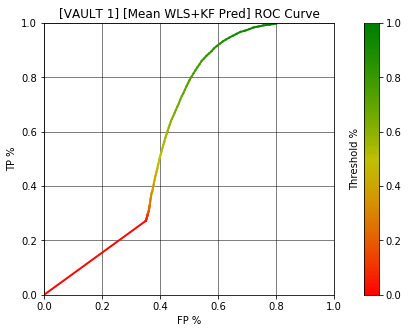
\includegraphics[width=8cm]{body/results/Graphs/JustSeries/1.PerformaceofMean/4.Combine/Raw/v1.png}
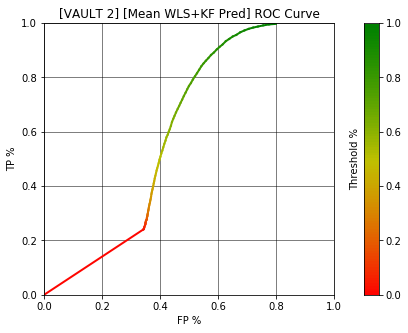
\includegraphics[width=8cm]{body/results/Graphs/JustSeries/1.PerformaceofMean/4.Combine/Raw/v2.png}
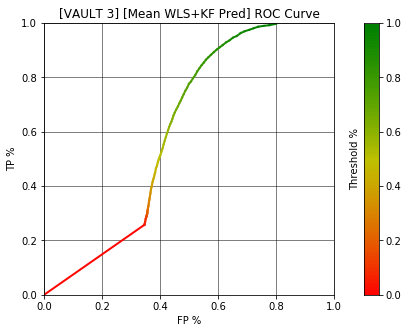
\includegraphics[width=8cm]{body/results/Graphs/JustSeries/1.PerformaceofMean/4.Combine/Raw/v3.png}
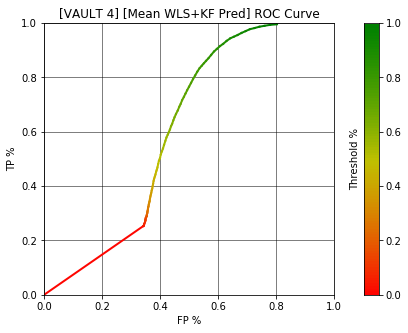
\includegraphics[width=8cm]{body/results/Graphs/JustSeries/1.PerformaceofMean/4.Combine/Raw/v4.png}
\caption{ROCs generated based on the average percent-fill prediction of all 15 of our KF's and all 15 of our WLS's combined for the entirety of each validation set. Top Left: Validation set 1. Top Right: Validation set 2. Bottom Left: Validation set 3. Bottom Right: Validation set 4.}
\label{fig:averageComb0}
\end{figure}

We thought averaging both the KF and WLS all together may improve the result. Figure \ref{fig:averageComb0} shows the outcome of averaging both together. As might be expected, the result was nearly identical to those previous with the initial flat section remaining and no improvement over the baseline evident.

\pagebreak

\begin{figure}[h]
\centering
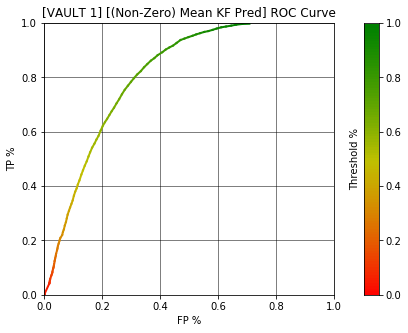
\includegraphics[width=8cm]{body/results/Graphs/JustSeries/1.PerformaceofMean/1.KF/Non-Zero/KFn0v1.png}
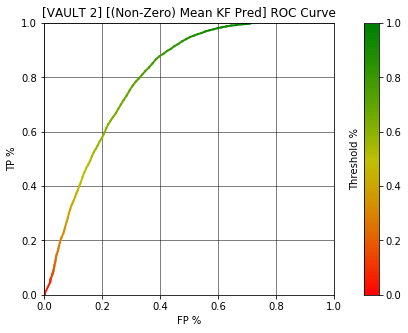
\includegraphics[width=8cm]{body/results/Graphs/JustSeries/1.PerformaceofMean/1.KF/Non-Zero/KFn0v2.png}
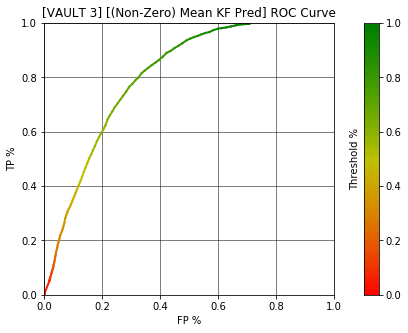
\includegraphics[width=8cm]{body/results/Graphs/JustSeries/1.PerformaceofMean/1.KF/Non-Zero/KFn0v3.png}
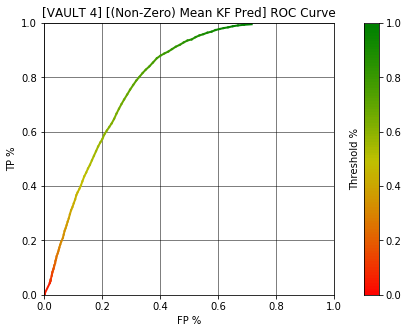
\includegraphics[width=8cm]{body/results/Graphs/JustSeries/1.PerformaceofMean/1.KF/Non-Zero/KFn0v4.png}
\caption{ROCs generated based on the average percent-fill prediction of all 15 of our KF's on the entirety of each validation set. Top Left: Validation set 1. Top Right: Validation set 2. Bottom Left: Validation set 3. Bottom Right: Validation set 4.}
\label{fig:averageKFn0}
\end{figure}

Figure \ref{fig:averageKFn0} is the same as Figure \ref{fig:averageKF0}, except it only uses ``non-zero'' data. We can plainly see significant performance improvements overall. At a False Positive Rate of 20\%, non-zero data performs 20\% better in terms of True Positive Rate. This would seem to bolster our theory that the abundance of dataless contests was detrimental for the average prediction.

\pagebreak

\begin{figure}[h]
\centering
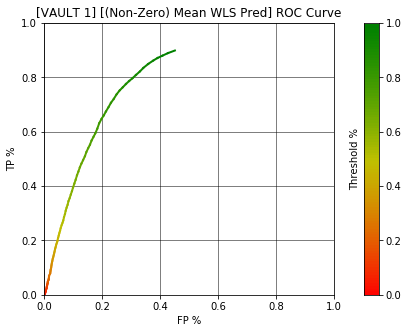
\includegraphics[width=8cm]{body/results/Graphs/JustSeries/1.PerformaceofMean/2.WLS/Non-Zero/v1.png}
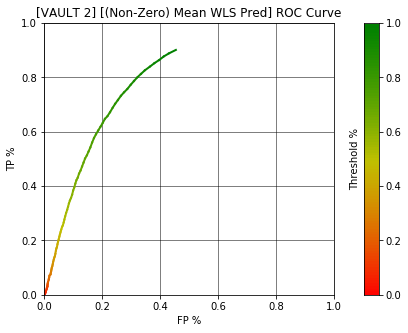
\includegraphics[width=8cm]{body/results/Graphs/JustSeries/1.PerformaceofMean/2.WLS/Non-Zero/v2.png}
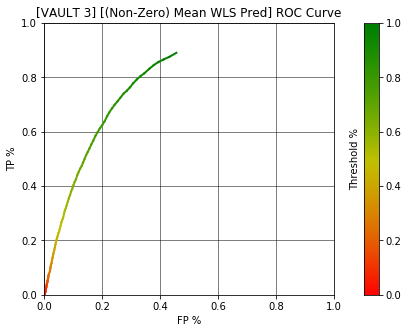
\includegraphics[width=8cm]{body/results/Graphs/JustSeries/1.PerformaceofMean/2.WLS/Non-Zero/v3.png}
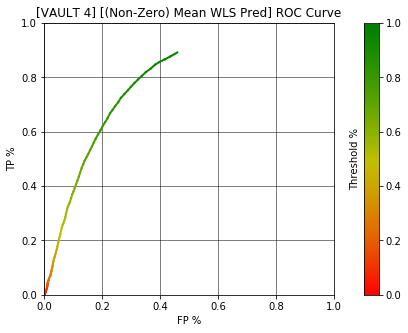
\includegraphics[width=8cm]{body/results/Graphs/JustSeries/1.PerformaceofMean/2.WLS/Non-Zero/v4.png}
\caption{ROCs generated based on the average percent-fill prediction of all 15 of our KF's on the entirety of each validation set. Top Left: Validation set 1. Top Right: Validation set 2. Bottom Left: Validation set 3. Bottom Right: Validation set 4.}
\label{fig:averageWLSn0}
\end{figure}

Figure \ref{fig:averageWLSn0} is the same as Figure \ref{fig:averageWLS0}, except it only uses ``non-zero'' data. Once again, we can see limiting the dataset leads to significant improvements over predicting on the entire set. In all 4 validation sets, the WLS curves can be seen to perform marginally better than those from the KF up to a False Positive rate of 0.3. This is unexpected, especially considering the KF performed better on the full sets. However, the WLS graphs also never reach a 100\% True Positive rate while the KF do. This is trade-off between the methods when averaging. A mroe direct comparison between the two can be seen in Figure \ref{fig:averageCompn0}.

\pagebreak

\begin{figure}[h]
\centering
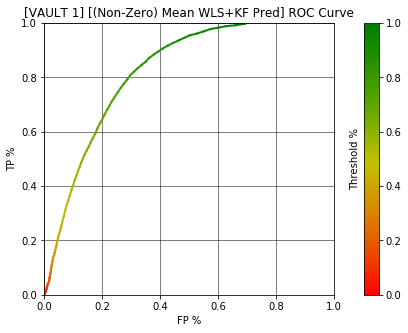
\includegraphics[width=8cm]{body/results/Graphs/JustSeries/1.PerformaceofMean/4.Combine/Non-Zero/v1.png}
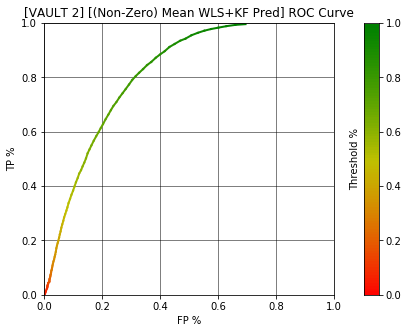
\includegraphics[width=8cm]{body/results/Graphs/JustSeries/1.PerformaceofMean/4.Combine/Non-Zero/v2.png}
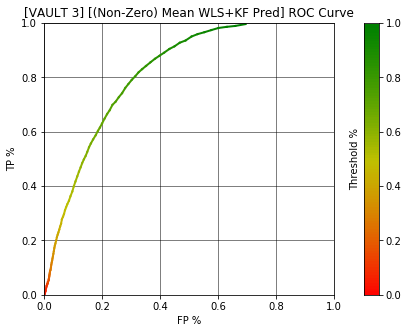
\includegraphics[width=8cm]{body/results/Graphs/JustSeries/1.PerformaceofMean/4.Combine/Non-Zero/v3.png}
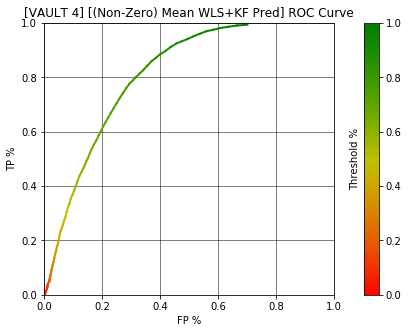
\includegraphics[width=8cm]{body/results/Graphs/JustSeries/1.PerformaceofMean/4.Combine/Non-Zero/v4.png}
\caption{ROCs generated based on the average percent-fill prediction of all 15 of our KF's and all 15 of our WLS's combined for the entirety of each validation set. Top Left: Validation set 1. Top Right: Validation set 2. Bottom Left: Validation set 3. Bottom Right: Validation set 4.}
\label{fig:averageCombn0}
\end{figure}

Figure \ref{fig:averageCombn0} shows the ROC generated by taking the average of all 15 KF's and WLS together. It's interesting to note that averaging both together produces a curve that seems to perform better than either method individually as if they somehow compensate for one another. Figure \ref{fig:averageCombn0} also appears in \ref{fig:averageCompn0} along side both the KF and WLS methods independently as well as the baseline.

\pagebreak

\begin{figure}[h]
\centering
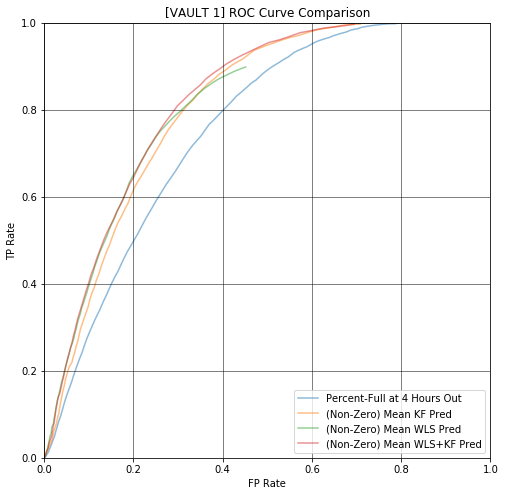
\includegraphics[width=7cm]{body/results/Graphs/JustSeries/1.PerformaceofMean/5.Compare/Non-Zero/v1.png}
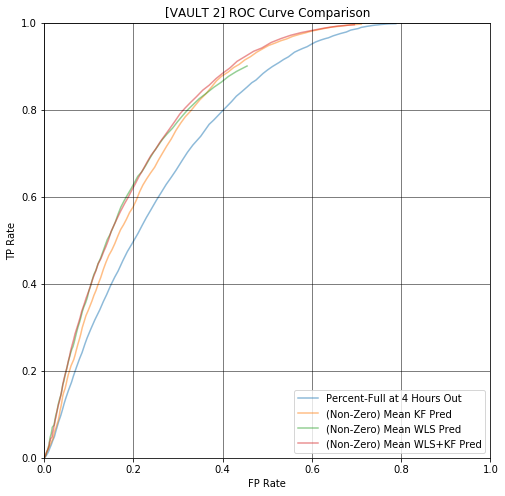
\includegraphics[width=7cm]{body/results/Graphs/JustSeries/1.PerformaceofMean/5.Compare/Non-Zero/v2.png}
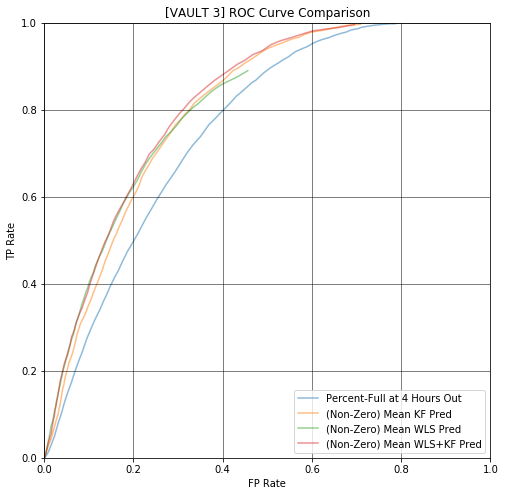
\includegraphics[width=7cm]{body/results/Graphs/JustSeries/1.PerformaceofMean/5.Compare/Non-Zero/v3.png}
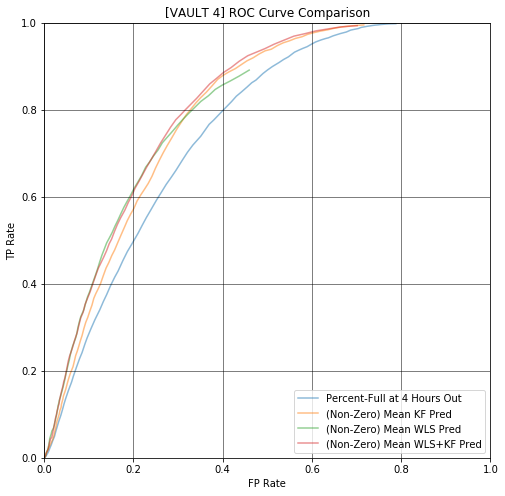
\includegraphics[width=7cm]{body/results/Graphs/JustSeries/1.PerformaceofMean/5.Compare/Non-Zero/v4.png}
\caption{ROCs generated based on the average percent-fill prediction of all 15 of our KF's on the entirety of each validation set. Top Left: Validation set 1. Top Right: Validation set 2. Bottom Left: Validation set 3. Bottom Right: Validation set 4.}
\label{fig:averageCompn0}
\end{figure}

From this, we can see by averaging our predictions (in the case of non-zero data) we already manage to outperform the baseline using time series data alone. However, considering the simplicity of the baseline that should not be considered a significant accomplishment. Seeing how well the ensemble of random forests did at predicting on just the Header data in Figure \ref{fig:metaonly}, we decided to investigate how well the ensemble could perform on time series predictions.

\pagebreak

Figures \ref{fig:ensembleKF0} - \ref{fig:ensembleTimeCombs} were generated based on the predictions from feeding the time series data into our KF and WLS with varying $Q$ and $\lambda$ parameters respectively. The final prediction was then found by feeding those predictions along with their respective $\alpha$ and $\beta$ parameters into out ensemble of random forests. The threshold being varied in these cases is once again the number of RFC required to flag a contest as a Positive (not filling).

\begin{figure}[h]
\centering
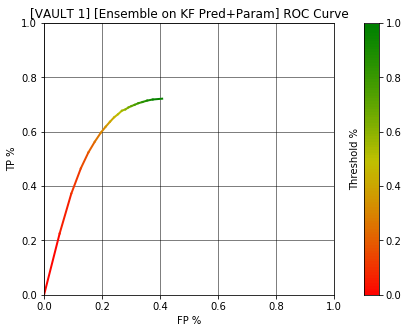
\includegraphics[width=8cm]{body/results/Graphs/JustSeries/2.PerformanceofEnsemble/1.KF/Raw/v1.png}
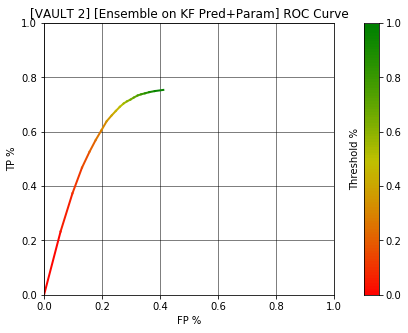
\includegraphics[width=8cm]{body/results/Graphs/JustSeries/2.PerformanceofEnsemble/1.KF/Raw/v2.png}
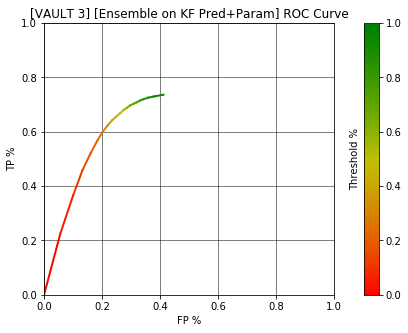
\includegraphics[width=8cm]{body/results/Graphs/JustSeries/2.PerformanceofEnsemble/1.KF/Raw/v3.png}
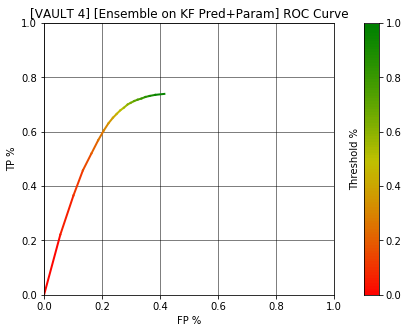
\includegraphics[width=8cm]{body/results/Graphs/JustSeries/2.PerformanceofEnsemble/1.KF/Raw/v4.png}
\caption{ROCs generated based on the ensemble prediction of the outputs of all 15 of our KF's (final entries prediction and model parameters) on the entirety of each validation set. Top Left: Validation set 1. Top Right: Validation set 2. Bottom Left: Validation set 3. Bottom Right: Validation set 4.}
\label{fig:ensembleKF0}
\end{figure}

Figure \ref{fig:ensembleKF0} was generated using only our 15 KF in our ensemble of random forests. Immediately, we can see the ensemble improves the predictive performance significantly compared to Figure \ref{fig:averageKF0}, without even having to delete dataless contests. A very similar result can be seen in Figure \ref{fig:ensembleWLS0} which shows the ROCs from using only WLS. While this is encouraging, we still wanted to look at how the ensemble performs on the ``non-zero'' data. 

\pagebreak

\begin{figure}[h]
\centering
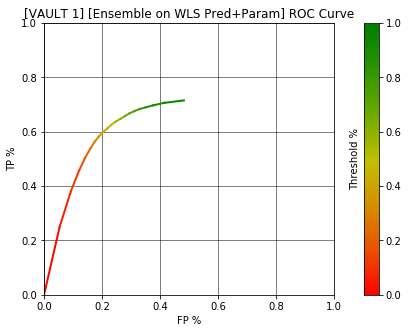
\includegraphics[width=8cm]{body/results/Graphs/JustSeries/2.PerformanceofEnsemble/2.LWS/Raw/v1.png}
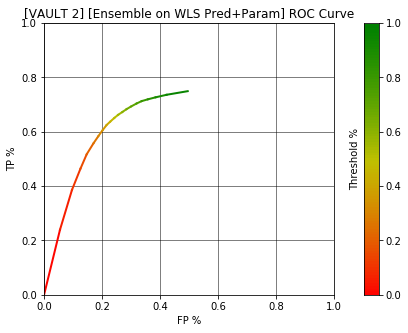
\includegraphics[width=8cm]{body/results/Graphs/JustSeries/2.PerformanceofEnsemble/2.LWS/Raw/v2.png}
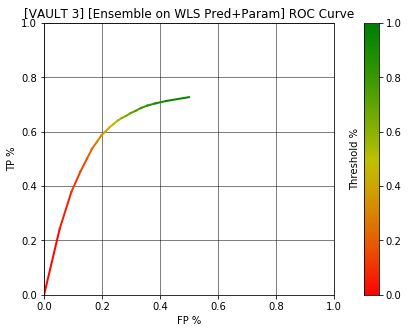
\includegraphics[width=8cm]{body/results/Graphs/JustSeries/2.PerformanceofEnsemble/2.LWS/Raw/v3.png}
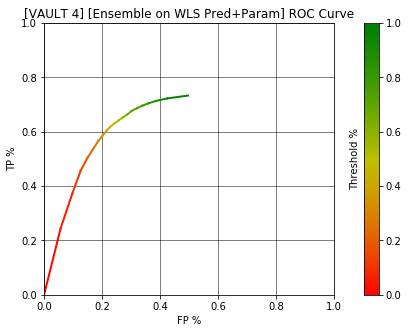
\includegraphics[width=8cm]{body/results/Graphs/JustSeries/2.PerformanceofEnsemble/2.LWS/Raw/v4.png}
\caption{ROCs generated based on the ensemble prediction of the outputs of all 15 of our WLS's (final entries prediction and model parameters) on the entirety of each validation set. Top Left: Validation set 1. Top Right: Validation set 2. Bottom Left: Validation set 3. Bottom Right: Validation set 4.}
\label{fig:ensembleWLS0}
\end{figure}

We repeated the same ensemble predictions as in Figures \ref{fig:ensembleKF0} and \ref{fig:ensembleWLS0} on only non-zero data. The results can be seen in Figure \ref{fig:ensembleTimeComps} along side the WLS adn KF methods individually and the baseline for reference.

\pagebreak

\begin{figure}[h]
\centering
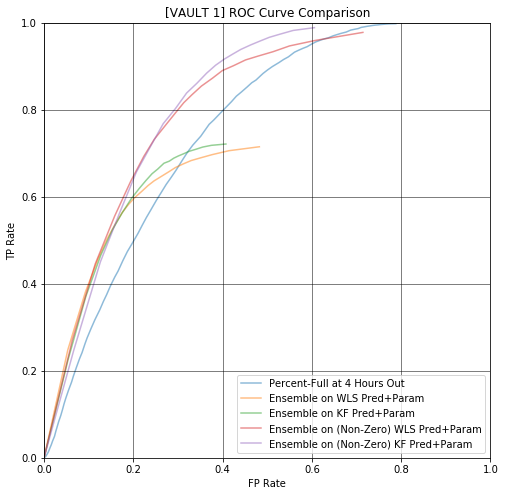
\includegraphics[width=7cm]{body/results/Graphs/JustSeries/2.PerformanceofEnsemble/3.Compare/v1.png}
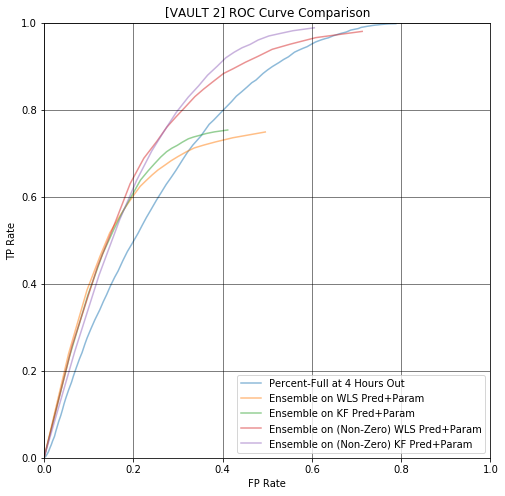
\includegraphics[width=7cm]{body/results/Graphs/JustSeries/2.PerformanceofEnsemble/3.Compare/v2.png}
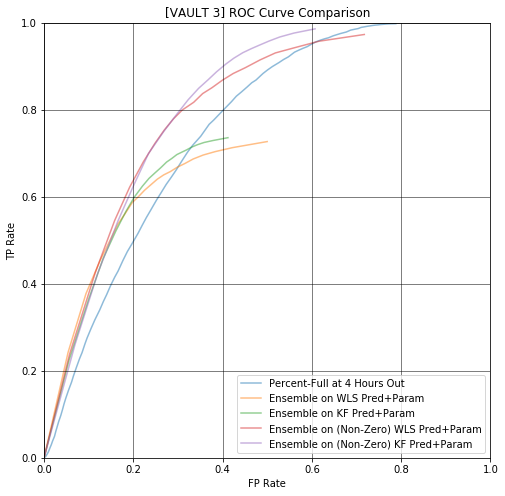
\includegraphics[width=7cm]{body/results/Graphs/JustSeries/2.PerformanceofEnsemble/3.Compare/v3.png}
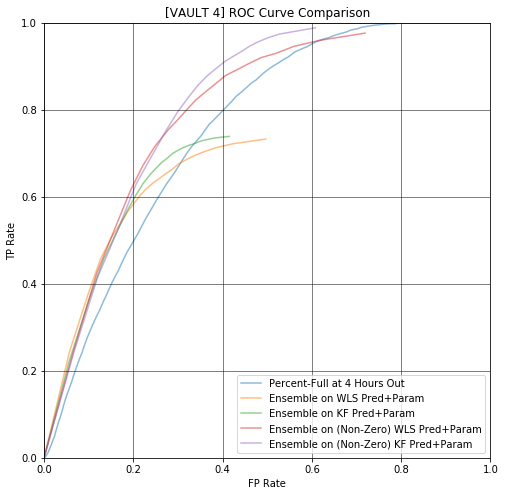
\includegraphics[width=7cm]{body/results/Graphs/JustSeries/2.PerformanceofEnsemble/3.Compare/v4.png}
\caption{Comparison of ROCs generated based on the ensemble prediction of the outputs of all 15 of our WLS's and KF's independently (final entries prediction and model parameters) on the entirety of each validation set and on just ``non-zero'' data. Top Left: Validation set 1. Top Right: Validation set 2. Bottom Left: Validation set 3. Bottom Right: Validation set 4.}
\label{fig:ensembleTimeComps}
\end{figure}

We can see that using non-zero data in the ensemble produces a negligible improvement in the prediction of both KF and WLs until a False Positive rate of 0.2. From there, the performance disparity grows rapidly. There also appears to be no significant difference in performance between WLS and KF, however, for small False Positive rates WLS does mildly better, while KF does better for False Positive rates above 0.3. In general, though, it seems all time series ensemble methods tend to outperform the baseline.

\pagebreak

\begin{figure}[h]
\centering
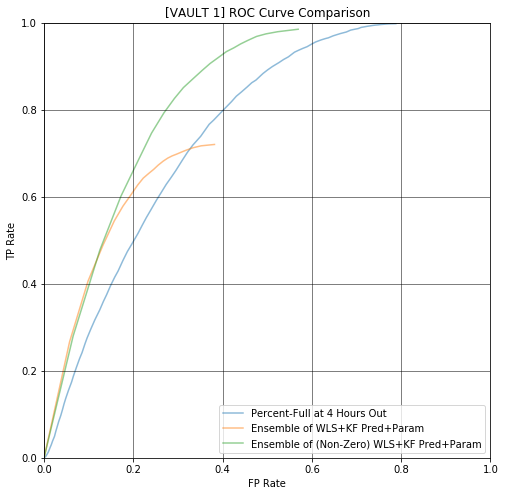
\includegraphics[width=7cm]{body/results/Graphs/JustSeries/2.PerformanceofEnsemble/4.Combine/Compare/v1.png}
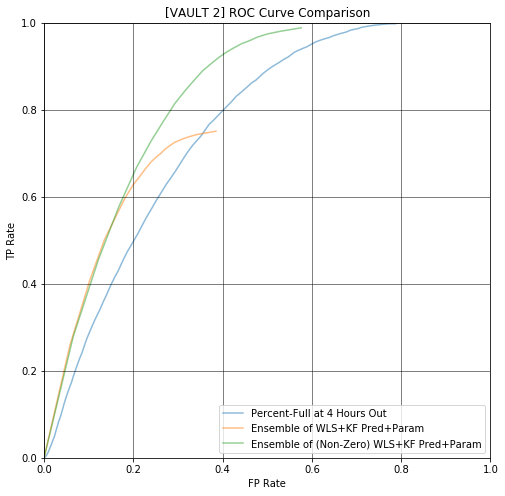
\includegraphics[width=7cm]{body/results/Graphs/JustSeries/2.PerformanceofEnsemble/4.Combine/Compare/v2.png}
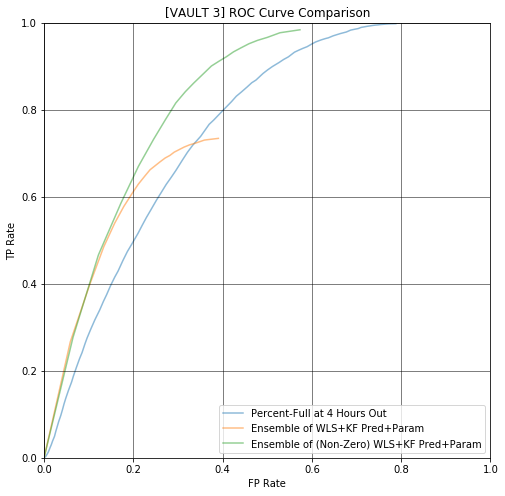
\includegraphics[width=7cm]{body/results/Graphs/JustSeries/2.PerformanceofEnsemble/4.Combine/Compare/v3.png}
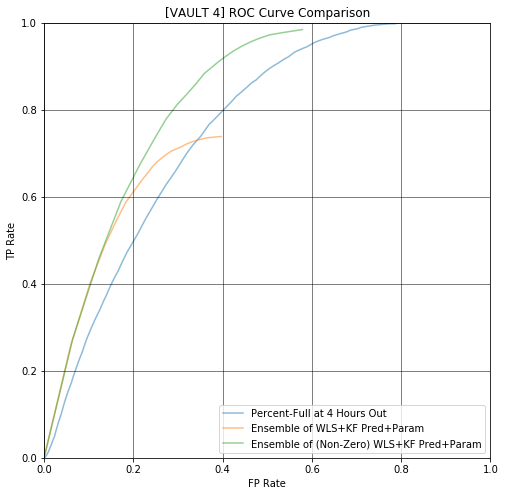
\includegraphics[width=7cm]{body/results/Graphs/JustSeries/2.PerformanceofEnsemble/4.Combine/Compare/v4.png}
\caption{Comparison of ROCs generated based on the ensemble prediction of the outputs of all 15 of our WLS's and KF's (final entries prediction and model parameters) together on the entirety of each validation set and on just ``non-zero'' data. Top Left: Validation set 1. Top Right: Validation set 2. Bottom Left: Validation set 3. Bottom Right: Validation set 4.}
\label{fig:ensembleTimeCombs}
\end{figure}

Random forests are known to be good at ignoring less useful data, meaning when provided more information they tend to perform strictly better or the same. With that in mind, we decided to see how well the ensemble could predict when given both the KF and WLS data. Figure \ref{fig:ensembleTimeCombs} shows a comparison of the outcomes. In general, the ensemble of both outperforms either individual ensemble, though it seems only marginally. Once again, the performance is far better when using only non-zero data.

\pagebreak